\chapter{Theoretical Background}
\label{ch:background}

This chapter lays the conceptual groundwork for the rest of the thesis. It opens by asking why distributed systems need a consensus mechanism at all, then works through the Raft algorithm step by step, with particular emphasis on leader election, log replication and the invariants that make the algorithm safe. The final part of the chapter turns to network topology theory, introducing the structural metrics that will later be used to compare how messages propagate across the five topologies under study.

\section{Distributed Systems and the Need for Consensus}

Following \citet{tanenbaum2017} and \citet{coulouris2011}, we take a distributed system to be a set of autonomous computers, each with its own memory, clock and failure mode, that cooperate closely enough that a user experiences them as a single machine. It is precisely this requirement -- many independent parts behaving as one -- that makes distributed systems simultaneously powerful and difficult to engineer.

Among the properties such a system must provide, consistency is usually the most important: once a client has written a value, it expects any later read to return that value, no matter which replica answers the request. Providing this guarantee is hard because the network linking the replicas may lose, delay or reorder messages, and because any replica can crash at any moment. Funnelling every request through a single designated node would sidestep the problem, but it would simply move the single point of failure onto that node. The standard alternative is to keep several copies of the state and run a consensus protocol that keeps every replica's view of the operation sequence in agreement.

Formally, consensus asks $n$ processes, each proposing a value, to agree on exactly one of those values, even though as many as $f$ of the processes may fail. \citet{lamport1998} characterises a correct consensus algorithm by four properties:

\begin{itemize}
    \item \textbf{Validity:} If every correct process proposes the same value, that value must be the one decided.
    \item \textbf{Agreement:} No two correct processes decide on different values.
    \item \textbf{Termination:} Every correct process eventually reaches a decision.
    \item \textbf{Integrity:} A process decides at most once.
\end{itemize}

A well-known impossibility result due to \citet{flp1985} shows that no deterministic algorithm running in a purely asynchronous system -- one where message delays are unbounded -- can guarantee all four properties if even a single process might fail. Practical algorithms work around this by abandoning pure asynchrony: they rely on timeouts to guess that a process has failed, and they assume the system is \emph{eventually synchronous}, meaning that message delays are bounded for long enough, often enough, that the algorithm can keep making progress.

\section{From Paxos to Raft}

Paxos held the position of default consensus algorithm for nearly two decades. \citet{lamport1998} introduced it, and the more accessible follow-up \citep{lamport2001} cemented its role as the theoretical basis for state-machine replication \citep{schneider1990}. Yet for all its elegance, Paxos has a long-standing reputation for being hard to follow and harder still to implement without subtle errors; systems that advertise Paxos compliance frequently diverge from the original specification in ways that introduce exactly such errors.

Raft, introduced by \citet{ongaro2014}, was a direct response to this state of affairs: ease of comprehension was treated as a design goal in its own right rather than an afterthought. Instead of presenting consensus as a single monolithic protocol, the authors split it into three pieces -- choosing a leader, replicating the log, and guaranteeing safety -- each of which can largely be studied on its own. Combined with clean interfaces between these pieces and a deliberate avoidance of optional optimisations, this structure is, by the authors' own user studies, considerably easier for newcomers to grasp than Paxos. The approach has proved popular in practice: Raft now underpins etcd \citep{etcd2024} (the configuration store behind Kubernetes), CockroachDB, HashiCorp Consul, TiKV and a range of other systems.

\section{The Raft Algorithm}

At the heart of Raft is a log that every server keeps a copy of. Each entry in this log encodes a command destined for the local state machine, and the algorithm's central job is to keep these copies in step: as long as every server applies the same commands in the same order, their state machines remain identical.

\subsection{Server States}

At any given moment, a Raft server occupies exactly one of three roles.

\begin{itemize}
    \item \textbf{Leader:} the sole server authorised to handle client requests; it replicates log entries to the rest of the cluster and keeps followers informed via periodic heartbeats.
    \item \textbf{Follower:} a passive role that only responds to RPCs initiated by a leader or a candidate, and never originates communication itself.
    \item \textbf{Candidate:} a temporary role adopted while a new leader is being chosen.
\end{itemize}

Every server begins life as a follower. If a follower hears nothing from a leader before its randomised election timeout elapses, it promotes itself to candidate and triggers an election.

\begin{figure}[H]
\centering
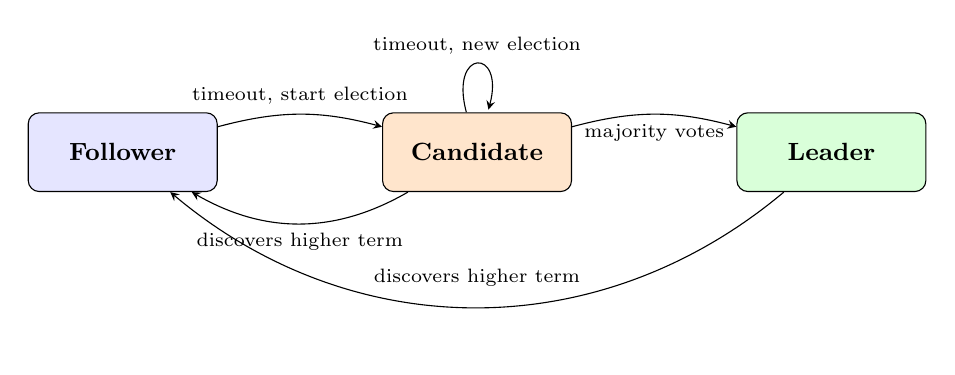
\begin{tikzpicture}[scale=1.0,
    state/.style={rectangle, draw, rounded corners, minimum width=2.4cm, minimum height=1cm, font=\small\bfseries, align=center},
    every edge/.style={draw, ->, >=stealth, font=\scriptsize}]
\node[state, fill=blue!10] (f) at (0,0) {Follower};
\node[state, fill=orange!20] (c) at (4.5,0) {Candidate};
\node[state, fill=green!15] (l) at (9,0) {Leader};

\draw[->, >=stealth] (f) edge[bend left=15] node[above, font=\scriptsize] {timeout, start election} (c);
\draw[->, >=stealth] (c) edge[bend left=15] node[below, font=\scriptsize] {majority votes} (l);
\draw[->, >=stealth] (c) edge[bend left=30] node[below, font=\scriptsize] {discovers higher term} (f);
\draw[->, >=stealth] (l) edge[bend left=40] node[above=4pt, font=\scriptsize] {discovers higher term} (f);
\draw[->, >=stealth] (c) edge[loop above] node[font=\scriptsize] {timeout, new election} (c);
\end{tikzpicture}
\caption{The three states of a Raft server and the transitions between them.}
\label{fig:raft_states}
\end{figure}

\subsection{Terms}

Time in Raft is partitioned into consecutively numbered \emph{terms} with no fixed duration. Every term opens with an attempt to elect a leader. When that attempt succeeds, the elected server governs the cluster until the term ends; when it fails -- typically because the vote was split between several candidates -- a new term begins immediately and the process repeats. Because every RPC is tagged with the sender's term number, terms double as a logical clock: any server that observes a term higher than its own immediately steps down to follower (if it was not one already) and adopts the higher term, allowing the cluster to discard stale leaders and outdated information without relying on synchronised clocks.

\subsection{Leader Election}

An election begins when a follower's timer runs out: the server switches to candidate, increments its term counter, casts a vote for itself, and sends a \texttt{RequestVote} RPC to every peer. Whichever candidate first gathers votes from a majority of the cluster becomes the new leader. Each server, however, votes for only the first candidate it encounters in a given term, and only if that candidate's log is at least as current as its own -- a rule known as the \emph{election restriction}. This restriction is what ensures that no entry already committed can ever be lost when leadership changes hands.

Should the vote split between competing candidates, the term ends without a leader and a fresh election follows. To keep such splits rare, and to guarantee that the cluster keeps making progress, Raft draws each server's election timeout from a random distribution -- commonly uniform between 150 and 300 milliseconds in production deployments.

\subsection{Log Replication}

After winning an election, a leader begins servicing client requests: each request becomes a new entry appended to the leader's log, which is then propagated to every follower via an \texttt{AppendEntries} RPC. Once a majority of servers have acknowledged storing the entry, it is considered \emph{committed}; the leader applies it to its own state machine and reports the result back to the client.

An \texttt{AppendEntries} RPC may carry any number of entries, including none at all -- an empty RPC serves purely as a heartbeat, and receiving one is enough for a follower to restart its election timer, so a healthy leader never triggers a needless election. To keep logs consistent across the cluster, every \texttt{AppendEntries} RPC also reports the index and term of the entry immediately preceding the new ones; a follower compares this against its own log and rejects the RPC if the two disagree, prompting the leader to retry with progressively earlier entries until a point where the logs agree is found.

\subsection{Safety}

The central safety guarantee of Raft is that, once an entry is committed, no later leader can ever undo it. Three properties work together to provide this guarantee. \emph{Election Safety} rules out more than one leader being elected within the same term, so there is never ambiguity about which server's log is authoritative at a given point in time. \emph{Leader Append-Only} restricts a leader to adding entries to its own log -- it is never permitted to modify or remove what is already there. \emph{Log Matching} states that whenever two servers' logs contain an entry with the same index and term, every entry preceding that point is also identical between the two logs. Together with the election restriction described above, these three properties are what make Raft's overwrite-free guarantee hold.

\subsection{Cluster Membership Changes}

Raft additionally specifies a joint-consensus mechanism for safely changing cluster membership while the system stays available. This thesis does not explore membership changes -- every simulation run uses a fixed number of nodes -- but it is worth noting briefly, since reconfiguration is a frequent source of subtle bugs in production deployments.

\section{Network Topology Theory}

By network topology we mean the pattern of links connecting the participating nodes. Graph-theoretically, this pattern can be represented as an undirected graph $G = (V, E)$, with $V$ the set of nodes and $E$ the set of bidirectional links between them. The shape of this graph governs three things that matter for our purposes: how quickly messages can travel between nodes, how resilient the network is when links or nodes fail, and how much redundant connectivity exists to route around such failures.

The analysis that follows draws on a small set of graph metrics, summarised below.

\begin{itemize}
    \item \textbf{Diameter} ($D$): the longest of all shortest paths between pairs of nodes, giving an upper bound on how many hops a message might need in the worst case.
    \item \textbf{Average path length} ($\bar{L}$): the shortest-path length averaged over every pair of nodes, a more representative proxy for typical latency than the diameter alone.
    \item \textbf{Node degree:} how many links attach to a given node. Topologies where every node has a low degree tend to offer little fault tolerance.
    \item \textbf{Connectivity:} the smallest number of node removals needed to split the graph into disconnected pieces. The higher this number, the more failures the network can absorb before fragmenting.
    \item \textbf{Edge count} ($|E|$): the total number of links in the graph, which roughly tracks both deployment cost and the number of paths messages can take in parallel.
\end{itemize}

\subsection{Star Topology}

In a Star topology, a single hub node connects directly to every other node, and no other links exist. An $n$-node Star therefore has $n-1$ edges, a diameter of two, and an average path length only slightly below two. Its weak point is the hub itself: if it fails, the cluster splits into isolated nodes.

\begin{figure}[H]
\centering
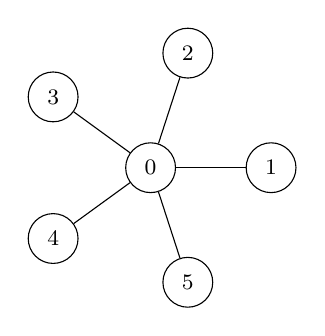
\begin{tikzpicture}[scale=0.85, every node/.style={circle, draw, minimum size=18pt, inner sep=0pt, font=\footnotesize}]
\node (h) at (0,0) {0};
\foreach \i/\angle in {1/0, 2/72, 3/144, 4/216, 5/288} {
    \node (n\i) at ({\angle}:1.8) {\i};
    \draw (h) -- (n\i);
}
\end{tikzpicture}
\caption{Star topology with five peripheral nodes connected to a central hub.}
\label{fig:topo_star}
\end{figure}

\subsection{Ring Topology}

A Ring connects every node to exactly two others so that the links trace out a single cycle. This gives an $n$-node Ring exactly $n$ edges and a diameter of $\lfloor n/2 \rfloor$, with the average path length scaling linearly in $n$ -- and so, consequently, does typical message latency as the cluster grows. A single link can fail without disconnecting the Ring (it degrades to a chain), but a second failure can partition it.

\begin{figure}[H]
\centering
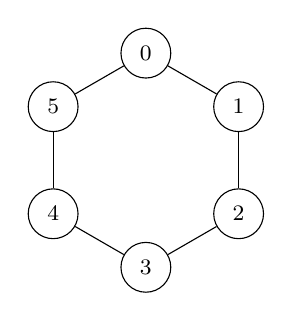
\begin{tikzpicture}[scale=0.85, every node/.style={circle, draw, minimum size=18pt, inner sep=0pt, font=\footnotesize}]
\foreach \i/\angle in {0/90, 1/30, 2/-30, 3/-90, 4/-150, 5/150} {
    \node (r\i) at ({\angle}:1.6) {\i};
}
\foreach \a/\b in {0/1, 1/2, 2/3, 3/4, 4/5, 5/0} {
    \draw (r\a) -- (r\b);
}
\end{tikzpicture}
\caption{Ring topology with six nodes connected in a closed loop.}
\label{fig:topo_ring}
\end{figure}

\subsection{Mesh Topology (Fully Connected)}

The Mesh topology connects every pair of nodes directly, giving $\binom{n}{2}$ edges, a diameter of one and an average path length of one as well. No other topology imposes fewer constraints on how messages travel, and none tolerates more link failures. The price is a quadratic number of links, which makes a physical Mesh impractical at scale -- but it remains a useful idealised upper bound against which the other topologies can be measured.

\begin{figure}[H]
\centering
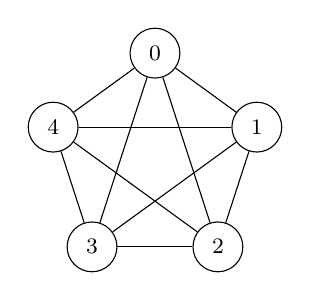
\begin{tikzpicture}[scale=0.85, every node/.style={circle, draw, minimum size=18pt, inner sep=0pt, font=\footnotesize}]
\foreach \i/\angle in {0/90, 1/18, 2/-54, 3/-126, 4/162} {
    \node (m\i) at ({\angle}:1.6) {\i};
}
\foreach \a in {0,1,2,3,4} {
    \foreach \b in {0,1,2,3,4} {
        \ifnum\a<\b \draw (m\a) -- (m\b); \fi
    }
}
\end{tikzpicture}
\caption{Mesh topology with five fully connected nodes; every pair shares an edge.}
\label{fig:topo_mesh}
\end{figure}

\subsection{Tree Topology (Binary Hierarchy)}

A Tree arranges its $n$ nodes hierarchically using $n-1$ edges; this thesis specifically uses a binary tree, for which a balanced layout gives a diameter of $O(\log n)$. The root and the nodes immediately below it carry disproportionate traffic and form natural bottlenecks. While this hierarchical structure scales well for broadcast-style communication, it is fragile in one specific sense: losing the root splits the rest of the tree into disconnected subtrees.

\begin{figure}[H]
\centering
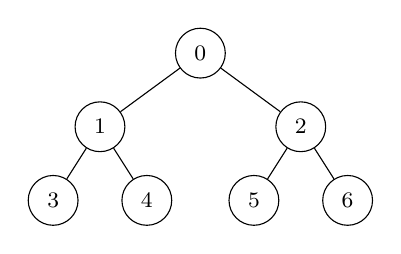
\begin{tikzpicture}[scale=0.85, level distance=1.1cm,
    level 1/.style={sibling distance=3cm},
    level 2/.style={sibling distance=1.4cm},
    every node/.style={circle, draw, minimum size=18pt, inner sep=0pt, font=\footnotesize}]
\node (root) {0}
    child {node {1}
        child {node {3}}
        child {node {4}}
    }
    child {node {2}
        child {node {5}}
        child {node {6}}
    };
\end{tikzpicture}
\caption{Binary Tree topology with seven nodes: node 0 is the root, leaves carry no children.}
\label{fig:topo_tree}
\end{figure}

\subsection{Bus Topology (Linear Chain)}

The Bus topology is simply a linear chain: $n$ nodes joined by $n-1$ edges, giving a diameter of $n-1$ and an average path length that grows linearly with cluster size. Any interior node that fails breaks the chain into two disconnected halves; only the two endpoint nodes can fail without partitioning the network. Despite this fragility, chain-like layouts persist in legacy industrial control networks, certain sensor-network deployments and long-haul fibre links.

\begin{figure}[H]
\centering
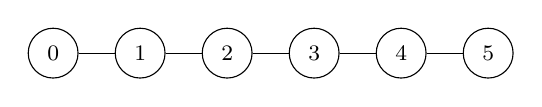
\begin{tikzpicture}[scale=0.85, every node/.style={circle, draw, minimum size=18pt, inner sep=0pt, font=\footnotesize}]
\foreach \i in {0,1,2,3,4,5} {
    \node (b\i) at (\i*1.3,0) {\i};
}
\foreach \a/\b in {0/1,1/2,2/3,3/4,4/5} {
    \draw (b\a) -- (b\b);
}
\end{tikzpicture}
\caption{Bus topology with six nodes arranged in a linear chain.}
\label{fig:topo_bus}
\end{figure}

\section{Related Work}

Existing performance evaluations of Raft tend to fall into two categories: those that optimise the implementation itself, and those that benchmark Raft against rival consensus algorithms. \citet{howard2020}, for instance, benchmark several Paxos and Raft variants side by side on commodity hardware, but model the network throughout as a uniform, low-latency LAN. Working under similarly uniform LAN assumptions, \citet{wang2017} modify Raft to pipeline log replication and report higher throughput as a result. \citet{larrea2018} examine leader election under unreliable network conditions, though their setting is Paxos rather than Raft. \citet{moraru2013} is closer in spirit to the present work, studying how geographic distribution affects EPaxos, while \citet{charapko2021} provide a broader survey of the consensus-implementation landscape.

What remains largely unexplored is how the shape of the underlying network -- as opposed to its raw latency -- affects Raft's behaviour. Simulations in the literature typically either assume a fully connected network or do not distinguish between topologies at all. This thesis addresses that gap by holding the consensus algorithm constant and systematically varying the topology under controlled, reproducible conditions.
